\begin{landscape}
    \chapter{Hodnoty ztrátové funkce modelu variačního autoenkodéru}
    \label{app:latent_space_development}

    \begin{figure}[H]
        \centering
        \subfloat[\centering Ztrátová funkce modelu po 200 epochách konverguje k hodnotě $\sim 137.5$.]{{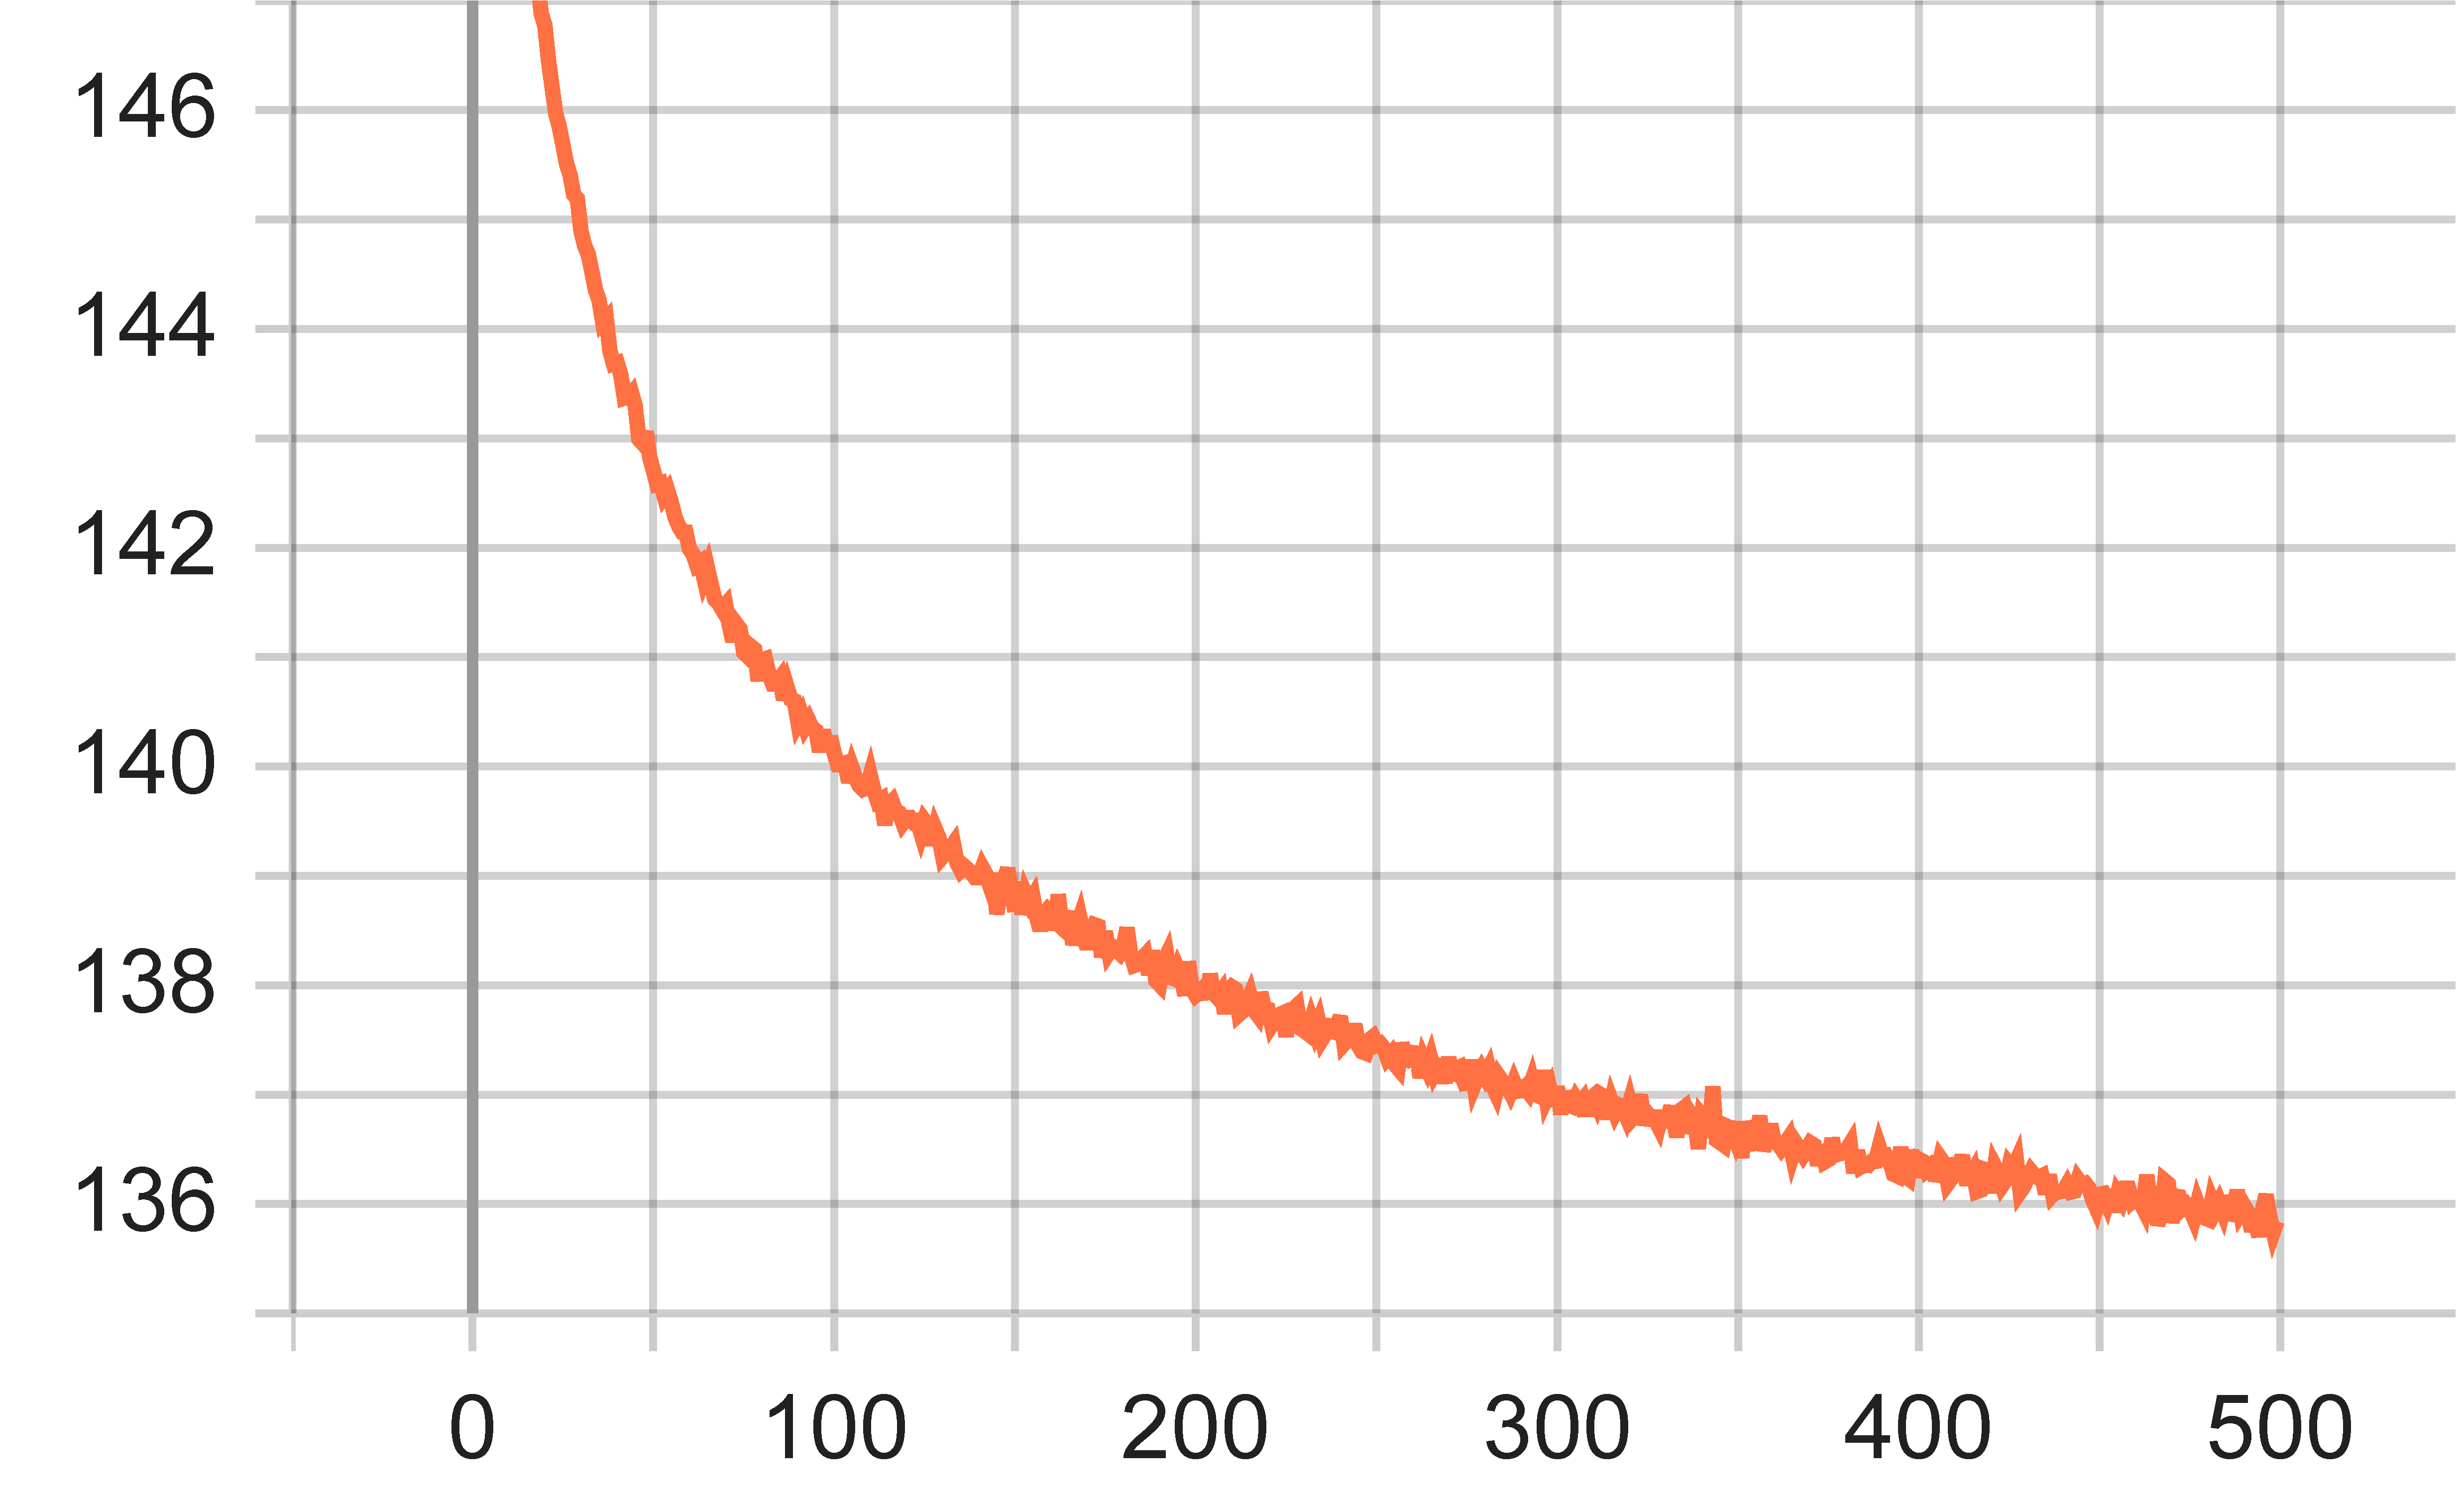
\includegraphics[width=0.43\textwidth]{figures/vae_model_total_loss_500_epochs_extended.pdf} }}
        \subfloat[\centering KL divergence modelu po 200 epochách konverguje k hodnotě $\sim 3.8$.]{{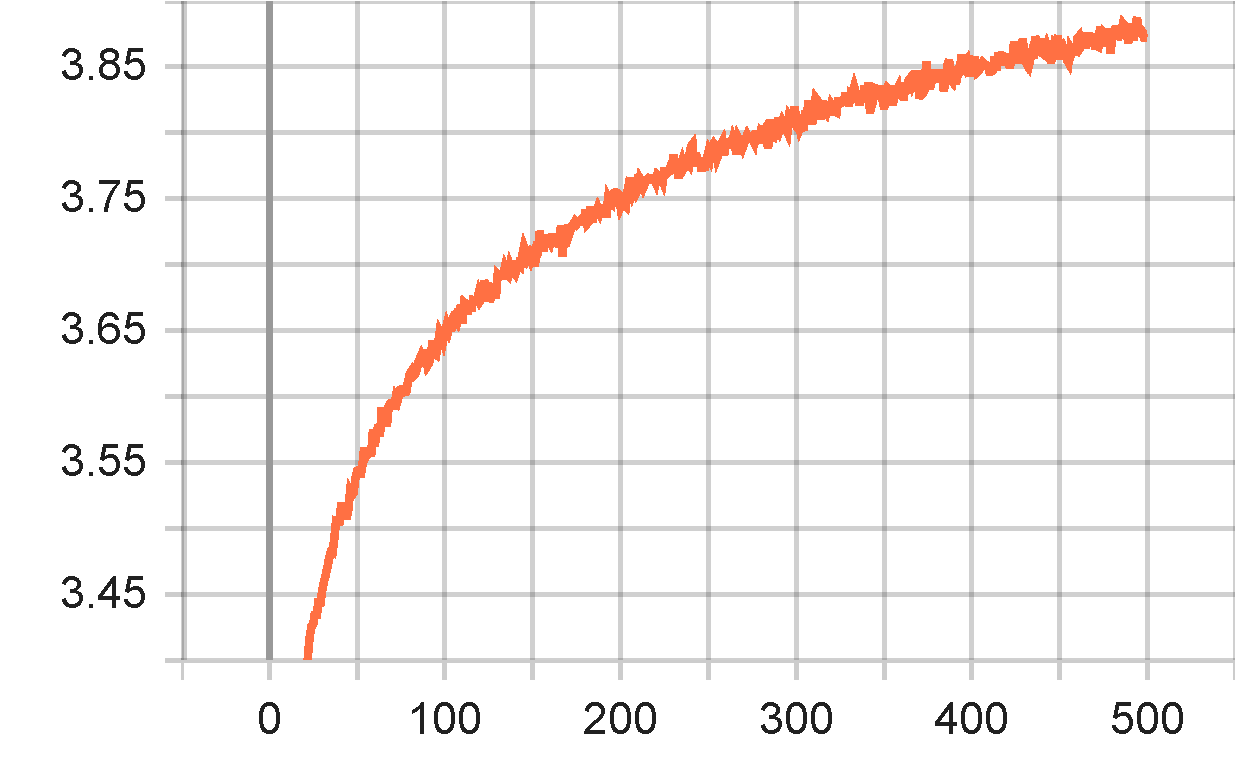
\includegraphics[width=0.43\textheight]{figures/vae_model_kl_loss_500_epochs.pdf } }}
        \subfloat[\centering Chyba rekonstrukce modelu po 200 epochách konverguje k hodnotě $\sim 133.7$.]{{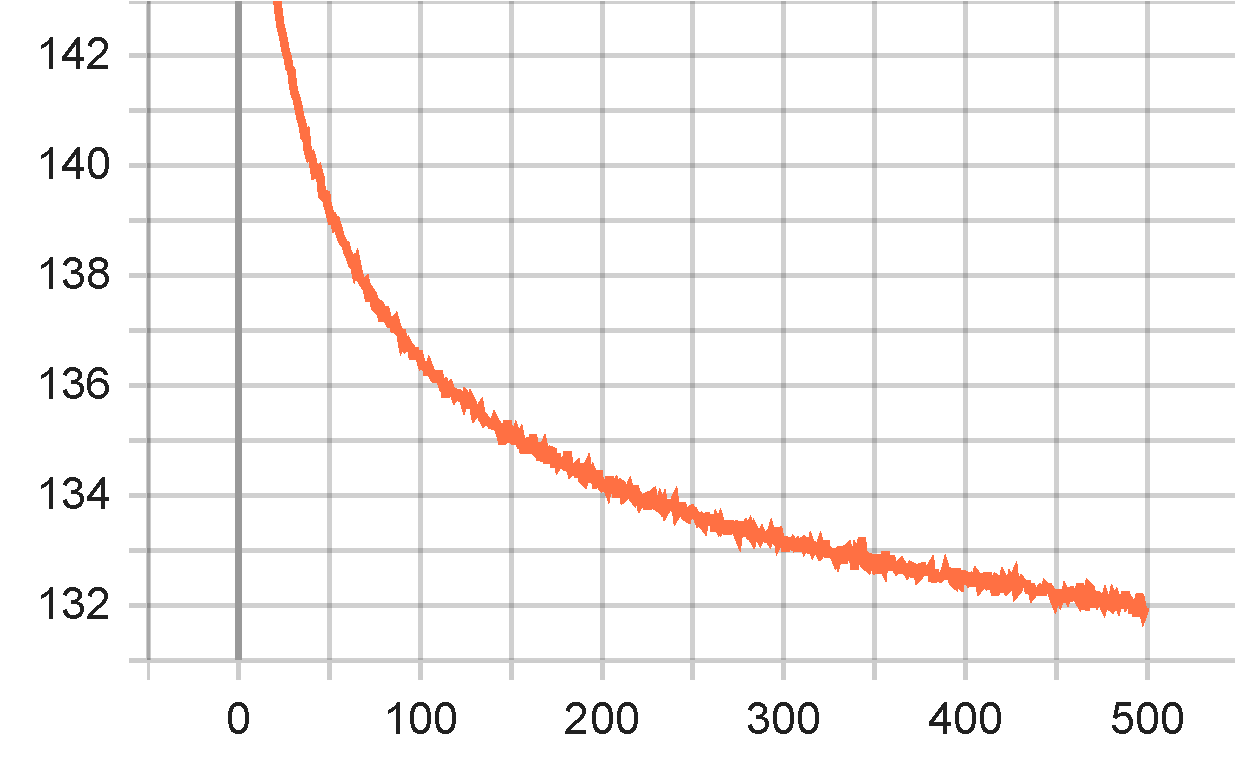
\includegraphics[width=0.43\textheight]{figures/vae_model_reconstruction_loss_500_epochs.pdf } }}
        \caption{Hodnota ztrátové funkce modelu variačního autoenkodéru po 200 epochách trénování.}
        \label{fig:example}
    \end{figure}

    \begin{figure}[H]
        \centering
        \subfloat[\centering Ztrátová funkce modelu po 500 epochách konverguje k hodnotě $\sim 135.8$.]{{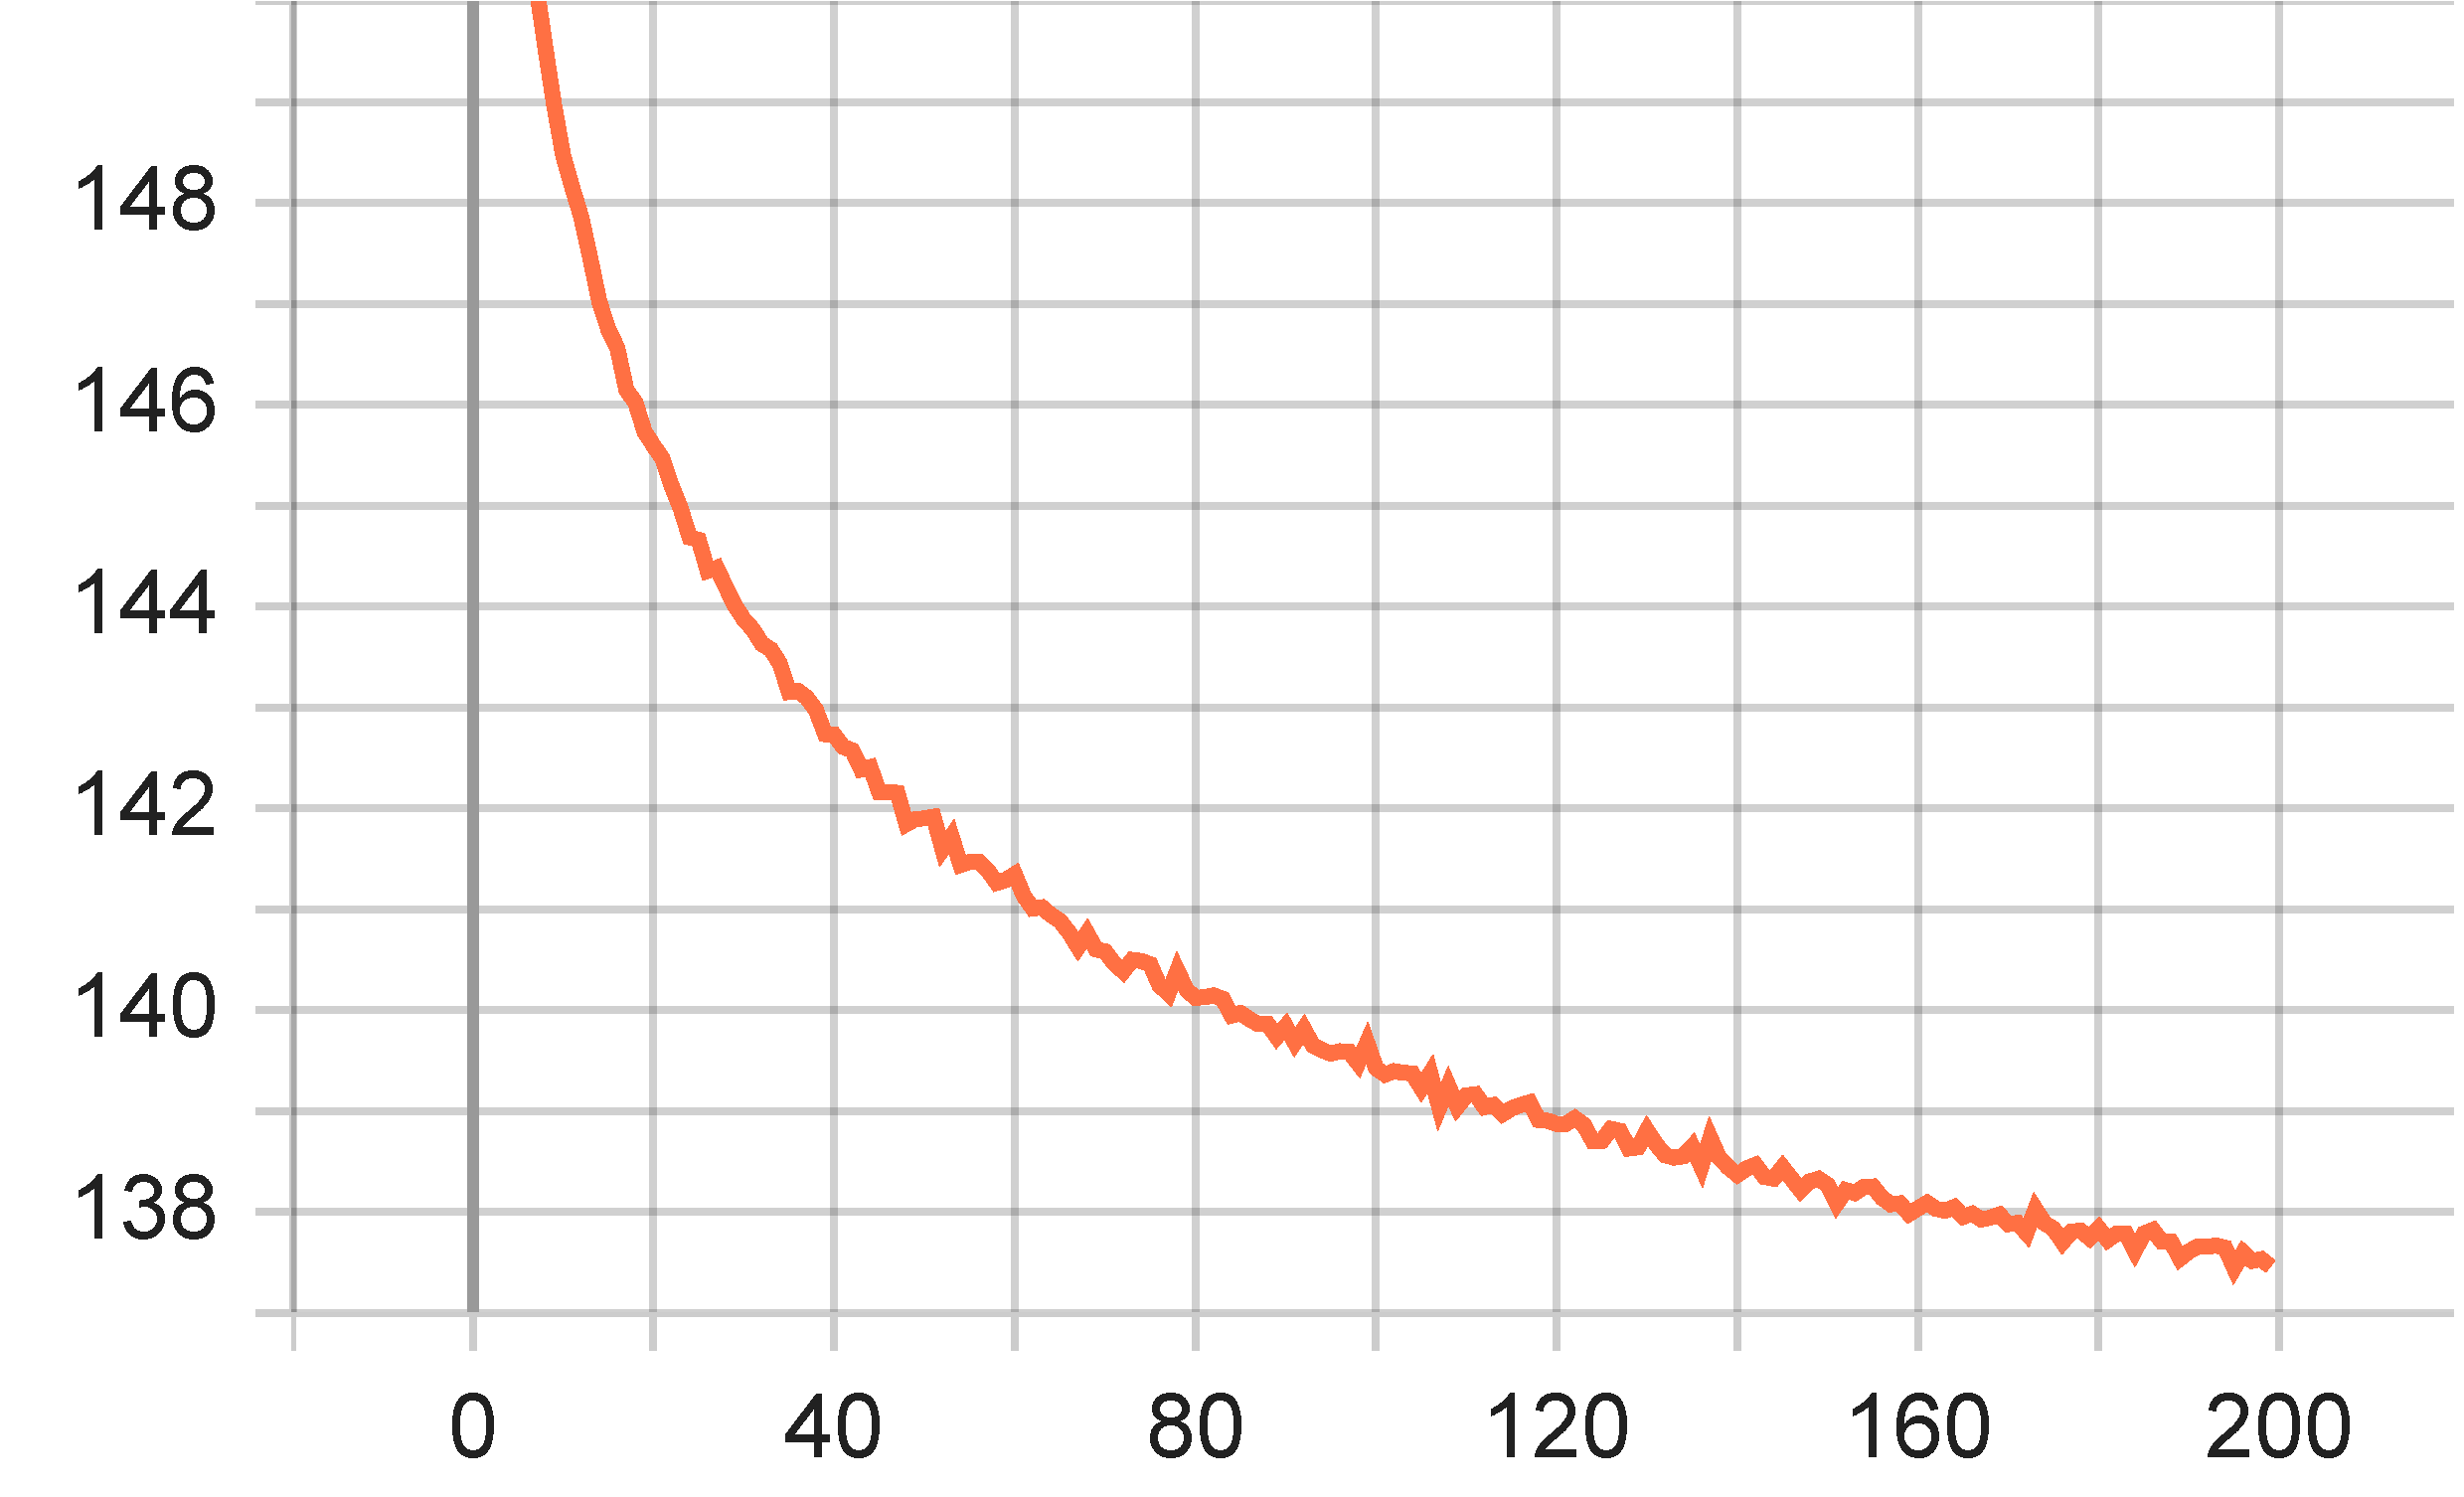
\includegraphics[width=0.43\textwidth]{figures/epoch_total_loss.pdf} }}
        \subfloat[\centering KL divergence modelu po 500 epochách konverguje k hodnotě $\sim 3.9$.]{{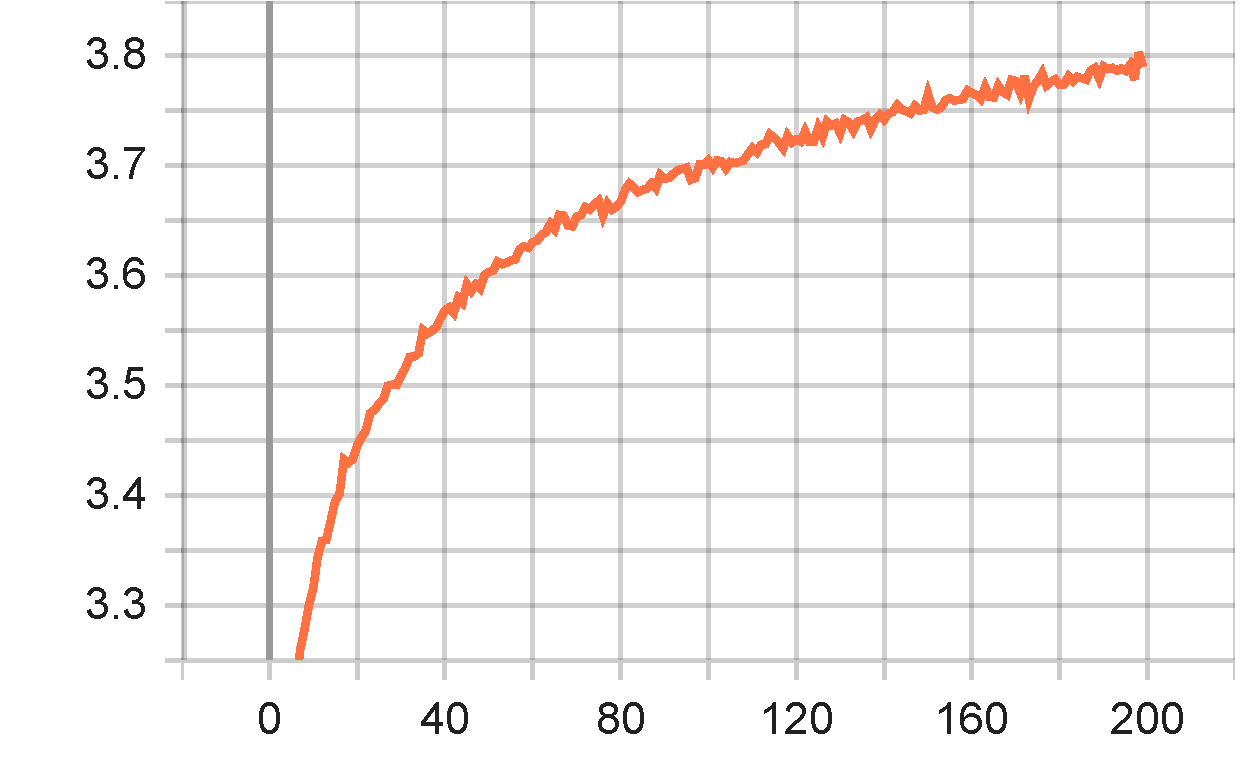
\includegraphics[width=0.43\textheight]{figures/epoch_kl_loss.pdf} }}
        \subfloat[\centering Chyba rekonstrukce modelu po 500 epochách konverguje k hodnotě $\sim 131.9$.]{{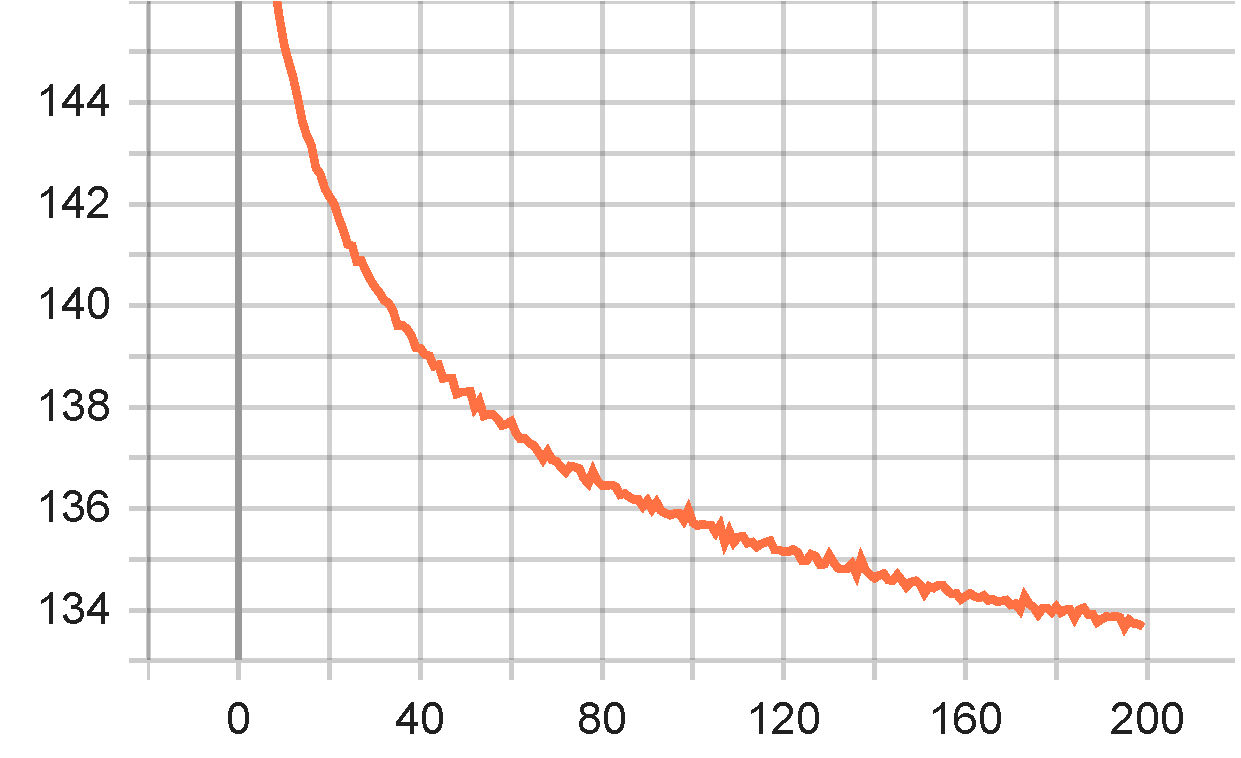
\includegraphics[width=0.43\textheight]{figures/epoch_reconstruction_loss.pdf} }}
        \caption{Hodnota ztrátové funkce modelu variačního autoenkodéru po 500 epochách trénování.}
        \label{fig:example}
    \end{figure}

\end{landscape}